\documentclass{article}
% \documentclass{beamer}
% \usetheme{Madrid}

%------------------------------
% used for href/url
\usepackage{hyperref}


% used for math fomulas
\usepackage{amsmath}

% used for tables
\usepackage{booktabs} % For better looking tables

% used for pictures
\usepackage{graphicx}
\usepackage{subcaption}
\usepackage{float}

% used for codes
\usepackage{listings}
\lstset{
  basicstyle=\ttfamily\footnotesize, % Set your code to be drawn with a monospaced font
  breaklines=true, % Enables line breaking
  frame=single % Adds a frame around the code
}

% used for Graph
\usepackage{adigraph}

% used for Bayesian Network
\usepackage{tikz}
\usetikzlibrary{bayesnet}

%------------------------------
% TODO 
\tolerance=10000
\emergencystretch=\maxdimen
\hyphenpenalty=10000
\hbadness=10000


\usepackage{silence}
\WarningFilter{latex}{Overfull \hbox}

%------------------------------



\title{MK's Notes for CIVL-4530 Geometric Design}
\date{2024-03-04}
\author{Michael Chen}

\begin{document}
  % \pagenumbering{gobble}
  % \maketitle
  % \newpage
  % \pagenumbering{arabic}
  % \setcounter{page}{29}
  \setcounter{section}{2}

  % todo ----------------------------------------
  % \tableofcontents
  % \newpage

  % ----------------------------------------
  \section{Sight Distance (SD)}
  \subsection{Objectives}
  \begin{enumerate}
    \item describe various types of sight distance
    \item determine sight distance requirements for stopping and passing maneuvers
  \end{enumerate}

  \subsection{key component of SD}
  \begin{enumerate}
    \item PRT: the perception-reaction time required to initiate a maneuver (pre-maneuver phase)
    \item MT: the time requried to safely complete a maneuver
  \end{enumerate}
  driver's eye - 3.5ft high\\
  Hazard - 2ft high \\


  \subsection{Sight Distance Types}
  \begin{enumerate}
    \item stopping sight distance (SSD)
    \item decision sight distance (DSD)
    \item passing sight distance (PSD)
    \item intersection sight distance (ISD)
  \end{enumerate}

  \subsection{SSD - stopping sight distance}
  SSD is a key input for geometric design, including horizontal and vertical alignment \\
  \\
  PRT includes: recognize an object + decide a stop + react and prepare to apply the brake \\
  Deceleration rate: $11.2ft/sec^{2}$, 10th percentile deceleration rate, by AASHTO \\
  \begin{align*}
    SSD & = D_{p-r} + D_{b}\\
        & \textbf{$D_{p-r}$: in ft, perception-reaction distance} \\
        & \textbf{$D_{b}$: in ft, braking distance} \\
        \\
    D_{p-r} & = 1.47 \times 2.5s \times v = 3.675v \\
            & \textbf{$D_{p-r}$: in ft, perception-reaction distance} \\
            & \textbf{v: in mi/h, design speed} \\
            \\
    D_{b} & = \frac{(v_{0})^2 - (v_{f})^2}{30(\frac{a}{g} \pm G)} \\
          & \textbf{$D_{b}$: in ft, braking distance}\\
          & \textbf{$v_{0}$: in mi/h, design speed} \\
          & \textbf{$v_{f}$: in mi/h, final velocity}\\
          & \textbf{a: 11.2 $ft/sec^2$, deceleration rate, by AASHTO, in [10, 15]} \\
          & \textbf{g: 32.2 $ft/sec^2$} \\
          & \textbf{f = a/g: 0.35 by ASSHTO, coefficient of friction, 0.7 for dry roads, 0.3-0.4 for wed roads} \\
          & \textbf{G: grade, e.g. down grade: -0.06} \\
  \end{align*}

  \subsection{SSD on vertical curve}
  crest curve: \\
    - Driver eye height: 3.5ft \\
    - Height of object in readway: 2.0ft \\
    \\
  sag curve: \\
    - headlight height: 2ft \\
    - headlight beam angle: 1 degree (departure from horizontal, suggest changing to 0.75 degree)


  \subsection{DSS - decision sight distance}
  For A or B (avoidance maneuvers): \\
  $DSD = 1.47V_{t} + 1.075(V^2/a)$ \\
  \\
  For C, D, and E: \\
  $DSD = 1.47V_{t}$ \\
  \\

  \subsection{DSS - decision sight distance}
  Decision sight distance for various conditions: \\
  \\
  Avoidance Maneuver A: Stop on rural road, t = 3.0 s\\
  Avoidance Maneuver B: Stop on urban road, t = 9.1 s\\
  \\
  Avoidance Maneuver C: Speed/path/direction change on rural road, t varies between 10.2 and 11.2 s \\
  Avoidance Maneuver D: Speed/path/direction change on suburban road, t varies between 12.1 and 12.9 s \\
  Avoidance Maneuver E: Speed/path/direction change on urban road, t varies between 14.0 and 14.5 s \\
  \\
  Source: AASHTO Green Book, 2011, Table 3-3\\



  \begin{table}[h!]
  \centering
  \caption{U.S. Customary Decision Sight Distance}
  \label{tab:us_customary_decision_sight_distance}
  \begin{tabular}{ccccccc}
  \toprule
  Design Speed (mph) & \multicolumn{5}{c}{Decision Sight Distance (ft)} &  \\
  \cmidrule(lr){2-6}
  & A & B & C & D & E & \\
  \midrule
  30 & 220 & 490 & 450 & 535 & 620 & \\
  35 & 275 & 590 & 525 & 625 & 720 & \\
  40 & 330 & 690 & 600 & 715 & 825 & \\
  45 & 395 & 800 & 675 & 800 & 930 & \\
  50 & 465 & 910 & 750 & 890 & 1030 & \\
  55 & 535 & 1030 & 865 & 980 & 1135 & \\
  60 & 610 & 1150 & 990 & 1125 & 1280 & \\
  65 & 695 & 1275 & 1050 & 1220 & 1365 & \\
  70 & 780 & 1410 & 1105 & 1275 & 1445 & \\
  75 & 875 & 1545 & 1180 & 1365 & 1545 & \\
  80 & 970 & 1685 & 1260 & 1455 & 1650 & \\
  \bottomrule
  \end{tabular}
  \end{table}

  \begin{table}[h!]
  \centering
  \caption{Metric Decision Sight Distance}
  \label{tab:metric_decision_sight_distance}
  \begin{tabular}{ccccccc}
  \toprule
  Design Speed (km/h) & \multicolumn{5}{c}{DSD (m)} \\
  \cmidrule(lr){2-6}
  & A & B & C & D & E \\
  \midrule
  50 & 70 & 155 & 145 & 170 & 195 \\
  60 & 95 & 195 & 170 & 205 & 235 \\
  70 & 115 & 325 & 200 & 235 & 275 \\
  80 & 140 & 280 & 230 & 270 & 315 \\
  90 & 170 & 325 & 270 & 315 & 360 \\
  100 & 200 & 370 & 315 & 355 & 400 \\
  110 & 235 & 420 & 330 & 380 & 430 \\
  120 & 265 & 470 & 360 & 415 & 470 \\
  130 & 305 & 525 & 390 & 450 & 510 \\
  \bottomrule
  \end{tabular}
  \end{table}

  \newpage

  \subsection{PSD - Passing sight distance}
  passing vehicle speed - passed vehicle speed $>=$ 12 mi/h\\
  \\
  On two-lane rural highways\\
  overtaking and returning to lane\\
  before opposing vehicle reaches passing vehicle\\


  \subsection{Passing sight distance assumptions - Green Book}
  \begin{enumerate}
    \item Speeds of passing and opposing vehicles equal the design speed
    \item Speed differential between the passing and passed vehicle is 12 mi/h
    \item Design vehicle is passenger car for all vehicles involved
    \item Perception-reaction time to decide to abort is 1 second
    \item Deceleration rate in abort maneuver is $11.2 ft/sec^2$
    \item Headway at end of maneuver is 1 second
  \end{enumerate}



  \begin{table}
  \centering
  \caption{U.S. Customary Assumed Speeds and Passing Sight Distance}
  \label{tab:us_customary_speeds}
  \begin{tabular}{cccc}
  \toprule
  Design Speed (mph) & Passed Vehicle (mph) & Passing Vehicle (mph) & Passing Sight Distance (ft) \\
  \midrule
  20 & 8  & 20 & 400 \\
  25 & 13 & 25 & 450 \\
  30 & 18 & 30 & 500 \\
  35 & 23 & 35 & 550 \\
  40 & 28 & 40 & 600 \\
  45 & 33 & 45 & 700 \\
  50 & 38 & 50 & 800 \\
  55 & 43 & 55 & 900 \\
  60 & 48 & 60 & 1000 \\
  65 & 53 & 65 & 1100 \\
  70 & 58 & 70 & 1200 \\
  75 & 63 & 75 & 1300 \\
  80 & 68 & 80 & 1400 \\
  \bottomrule
  \end{tabular}
  \end{table}
  
  \begin{table}[h!]
  \centering
  \caption{Metric Passing Sight Distance}
  \label{tab:metric_passing_sight_distance}
  \begin{tabular}{cccc}
  \toprule
  Design Speed (km/h) & Assumed Speeds Passed Vehicle (km/h) & Passing Vehicle (km/h) & PSD (m) \\
  \midrule
  30 & 11 & 30 & 120 \\
  40 & 21 & 40 & 140 \\
  50 & 31 & 50 & 160 \\
  60 & 41 & 60 & 180 \\
  70 & 51 & 70 & 210 \\
  80 & 61 & 80 & 245 \\
  90 & 71 & 90 & 280 \\
  100 & 81 & 100 & 320 \\
  110 & 91 & 110 & 355 \\
  120 & 101 & 120 & 395 \\
  130 & 111 & 130 & 440 \\
  \bottomrule
  \end{tabular}
  \end{table}
  
  \subsection{Intersection Sight Distance - ISD} 
  Sighting Rod - 3.5 feet height
  Target Rod - 4.25 feet height
  Observer - 10 feet behind stop bar

  \begin{figure}
    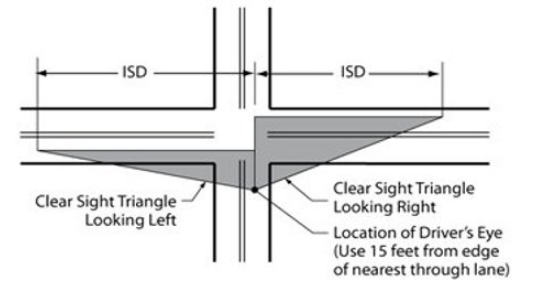
\includegraphics[width=0.7\linewidth]{ISD_leftturn.png}
    \caption{ISD - Left Turn}
    \label{fig:image-isd-leftturn}
  \end{figure}

  \begin{figure}
    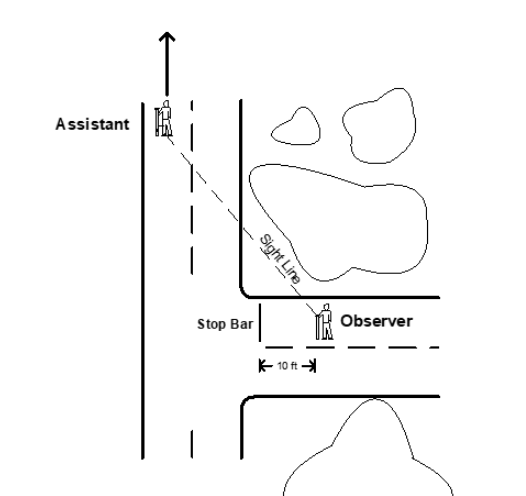
\includegraphics[width=0.7\linewidth]{ISD_observer.png}
    \caption{ISD - Observer}
    \label{fig:image-isd-observer}
  \end{figure}

  \subsection{Intersection sight distance fomulas}

  \begin{align*}
    ISD & = 1.47 V_{major} \cdot t_g \\
    & V_{majro}: \text{in mph, design speed of major road} \\
    & t_g: \text{in seconds, time gap for minor road vehicle to enter the major road} \\
  \end{align*}

  \subsection{ISD - left turn}
  \begin{tabular}{|l|c|}
    \hline
    \textbf{Design vehicle} & \textbf{$t_g$ in seconds, LT Time Gap} \\
    \hline
    Passenger car & 7.5 \\
    \hline
    Single-unit truck & 9.5 \\
    \hline
    Combination truck & 11.5 \\
    \hline
  \end{tabular}

  \begin{enumerate}
    \item \textbf{Left turn and multilanes}: If requiring to cross one more lane, +0.5s for passenger cars, +0.7s for trunks.
    \item \textbf{Grade of minor road}: If the approach grade $> +3\%$, add 0.2s per additional grade.
  \end{enumerate}

  \subsection{ISD - right turn}
  \begin{tabular}{|l|c|}
  \hline
  \textbf{Design vehicle} & \textbf{$t_g$ in seconds, RT time gap}\\
  \hline
  Passenger car & 6.5 \\
  \hline
  Single-unit truck & 8.5 \\
  \hline
  Combination truck & 10.5 \\
  \hline
  \end{tabular}

  \begin{enumerate}
    \item \textbf{right turn and multilanes}: If requiring to cross one more lane, +0.5s for passenger cars, +0.7s for trunks.
    \item \textbf{Grade of minor road}: If the approach grade $> +3\%$, add 0.1s per additional grade.
  \end{enumerate}


  % ----------------------------------------
  \subsection{Terms}

  \subsection{Rules}

  \subsection{Formulas}

  \subsection{Reference}


% --------------------------------------
\end{document}
